\documentclass{article}

\usepackage{amsmath}
\usepackage{amscd}
\usepackage[utf8]{inputenc}

\usepackage{Sweave}
\begin{document}
\Sconcordance{concordance:example.tex:example.Rnw:%
1 6 1 1 0 15 1 1 2 7 0 1 2 2 1 1 2 1 0 7 1 3 0 1 2 4 1 1 2 1 0 1 1 3 0 %
1 2 1 1 1 -3 1 7 8 1}


\title{An Sweave Demo}
\author{Charles J. Geyer}
\maketitle

This is a demo for using the \verb@Sweave@ command in R.  To
get started make a regular \LaTeX\ file (like this one) but
give it the suffix \verb@.Rnw@ instead of \verb@.tex@ and then
turn it into a \LaTeX\ file (\verb@foo.tex@) with the (unix) command
\begin{verbatim}
R CMD Sweave foo.Rnw
\end{verbatim}

Well, we can now include R in our document.  Here's a simple example
\begin{Schunk}
\begin{Sinput}
> 2 + 2
\end{Sinput}
\begin{Soutput}
[1] 4
\end{Soutput}
\end{Schunk}

Plots get a little more complicated.  First we make something to plot
(simulate regression data).
\begin{Schunk}
\begin{Sinput}
> n <- 50
> x <- seq(1, n)
> a.true <- 3
> b.true <- 1.5
> y.true <- a.true + b.true * x
> s.true <- 17.3
> y <- y.true + s.true * rnorm(n)
> out1 <- lm(y ~ x)
\end{Sinput}
\end{Schunk}
(for once we won't show the code chunk itself, look at \verb@foo.Rnw@
if you want to see what the actual code chunk was).

Figure~\ref{fig:one} (p.~\pageref{fig:one})
is produced by the following code
\begin{Schunk}
\begin{Sinput}
> plot(x, y)
> abline(out1)
\end{Sinput}
\end{Schunk}
\begin{figure}
\begin{center}
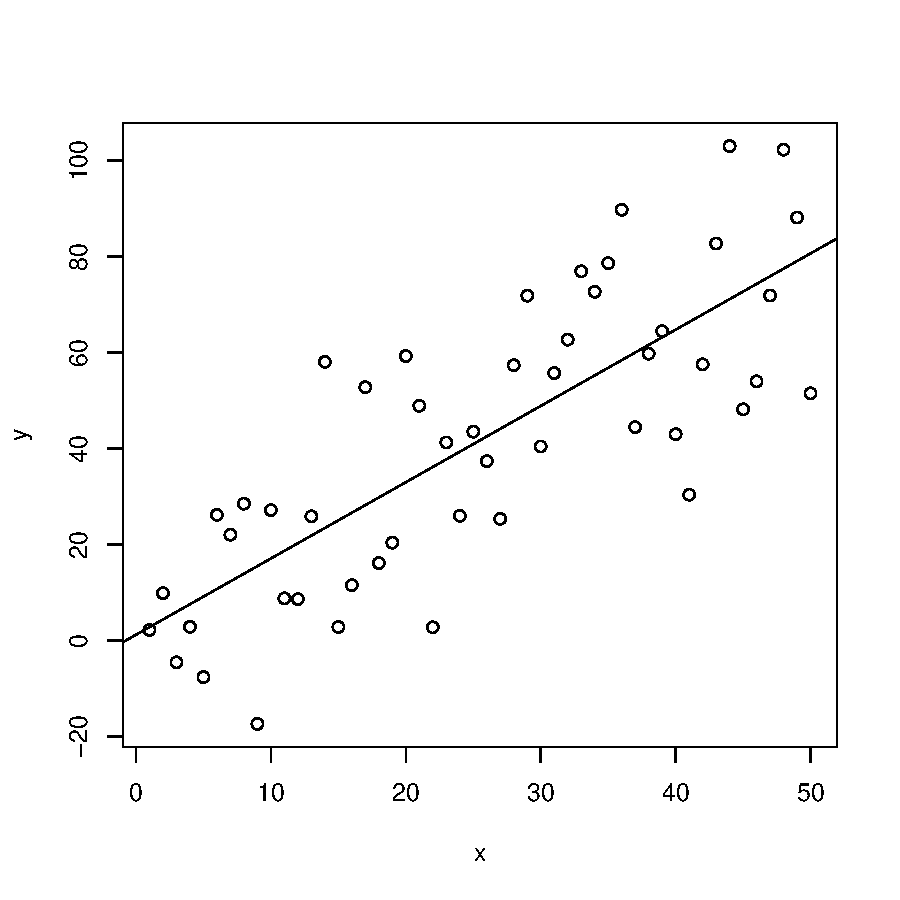
\includegraphics{example-fig1}
\end{center}
\caption{Scatter Plot with Regression Line}
\label{fig:one}
\end{figure}
Note that \verb@x@, \verb@y@, and \verb@out1@ are remembered from
the preceding code chunk.  We don't have to regenerate them.
All code chunks are part of one R ``session''.

\end{document}
